\chapter{Modelagem geral do sistema} \label{chap:modelagem} % 4.

Tendo esclarecido sobre as questões gerais do trabalho e da área de estudo. Agora nos aprofundaremos um pouco mais na modelagem e criação de diagramas que ilustrem o funcionamento geral do sistema e a forma como se dará a execução da metodologia proposta.

\section{Estágios de execução} % 4.1.

Em seu trabalho de aplicação prática, \citeonline{miranda_udpskeduler_2012} estruturaram estágios que compõem o processo necessário para que enfim se alcance a definição de tabelas horárias finais.

\begin{CenteredFigure}
  \caption{Estágios para a obtenção de grade horária ótima}
  \label{fig:geral}
  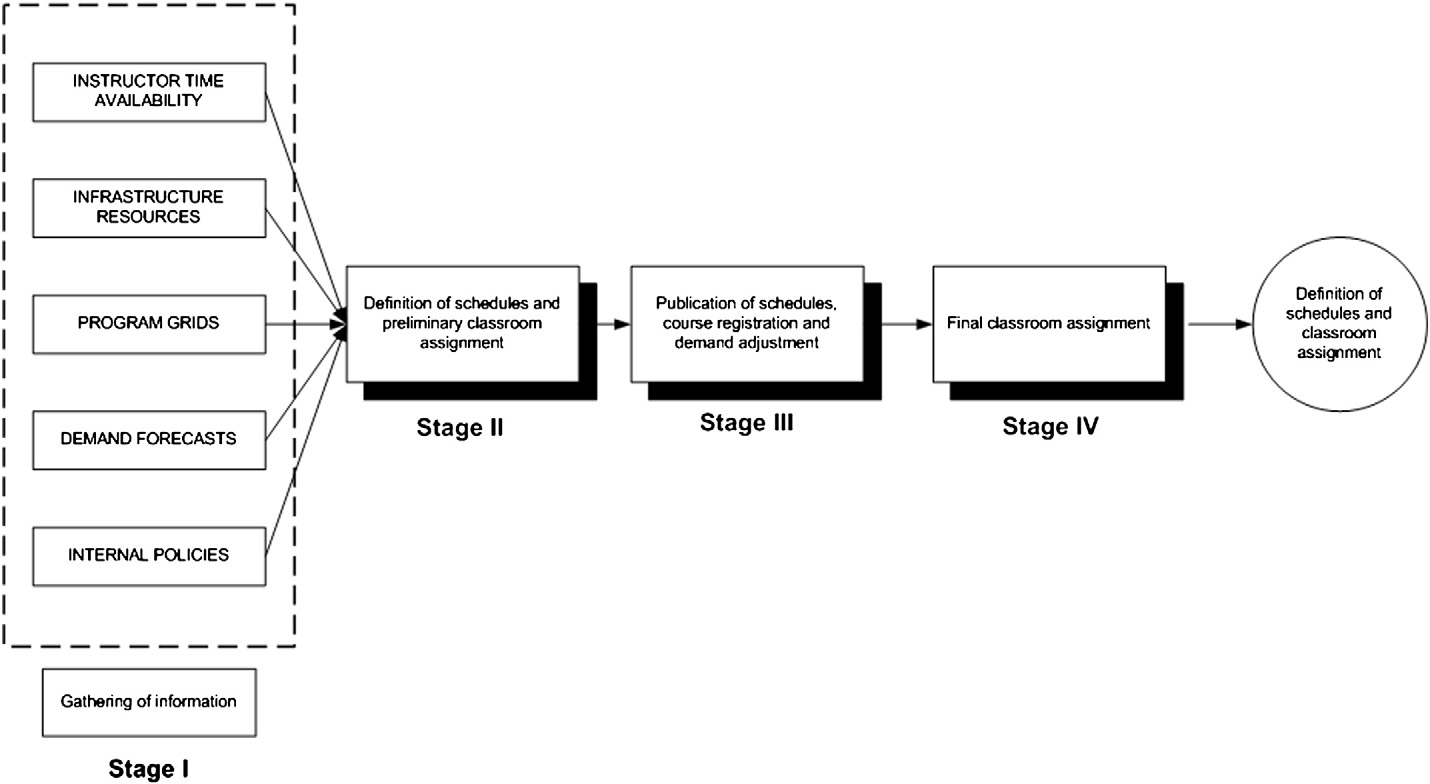
\includegraphics[width=\textwidth]{files/img/2.02!4-modelagem/Arquitetura-UDP}
  \legend{Fonte: \citeonline{miranda_udpskeduler_2012}}
\end{CenteredFigure}

Na \autoref{fig:geral}, estão dispostos 4 estágios principais. O primeiro dispõe da aquisição de informações, sendo elas a disponibilidade do profesor, os recuresos da infraestrutura, as grades dos cursos, as estimativas de demanda e as políticas internas. No segundo estágio são definidas grades horárias preliminares com atribuição preliminar das salas. No terceiro, os alunos se inscrevem e a demanda é ajustada, por fim, no quarto estágio, ocorre a alocação final das salas. Com sua conclusão, são definidos as grades horárias finais junto com as respectivas salas.

Seguindo seu exemplo, te

\section{Iteração} % 4.2.

Para se alcançar uma alta satisfação por parte dos \textit{stakeholders}, vê-se necessária a constante interação com os mesmos. Para isto, será seguida a estrutura utilizada por \citeonline{andre_interaction_2018}.

\begin{MyCenteredFigure}
  \caption{Etapas do Design de Interação}
  \label{fig:IxD}
  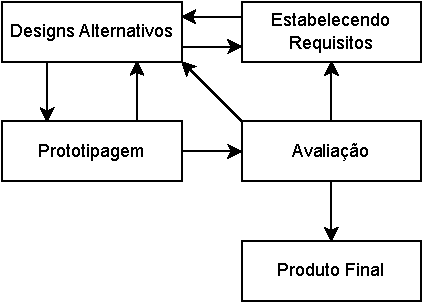
\includegraphics{files/img/2.02!4-modelagem/Arquitetura-IxD.drawio}
\end{MyCenteredFigure} % University

Seguindo o conceito do Design de Interação, a \autoref{fig:IxD} ilustra o ciclo de ações a serem tomadas durante o desenvolvimento do sistema, caso este venha a ser necessário. Nesse modelo de pesquisa, os \textit{stakeholders} serão consultados continuamente enquanto lhes for apresentados protótipos do sistema, para que assim informem quanto às suas percepções. Esta dinâmica tem como finalidade encontrar um design tal que seja adequado aos desejos e necessidades de seus usuários. Pois, considerando que para que o sistema seja efetivo, é necessário que ele seja aceito e utilizado pelos usuários finais.

\section{Funcionamento} % 4.3.

REESCREVER

\section{Modelo de Banco de Dados} \label{sec:ModelagemBD} % 4.4.

Considerando as informações necessárias para o presente trabalho, e também o preparo de campo para potenciais aplicações futuras, foi elaborado um diagrama conceitual de banco de dados, que pode ser visto na \autoref{fig:DiagramConceitual}.

\begin{MyCenteredFigure}
  \caption{Diagrama Conceitual do banco de dados}
  \label{fig:DiagramConceitual}
  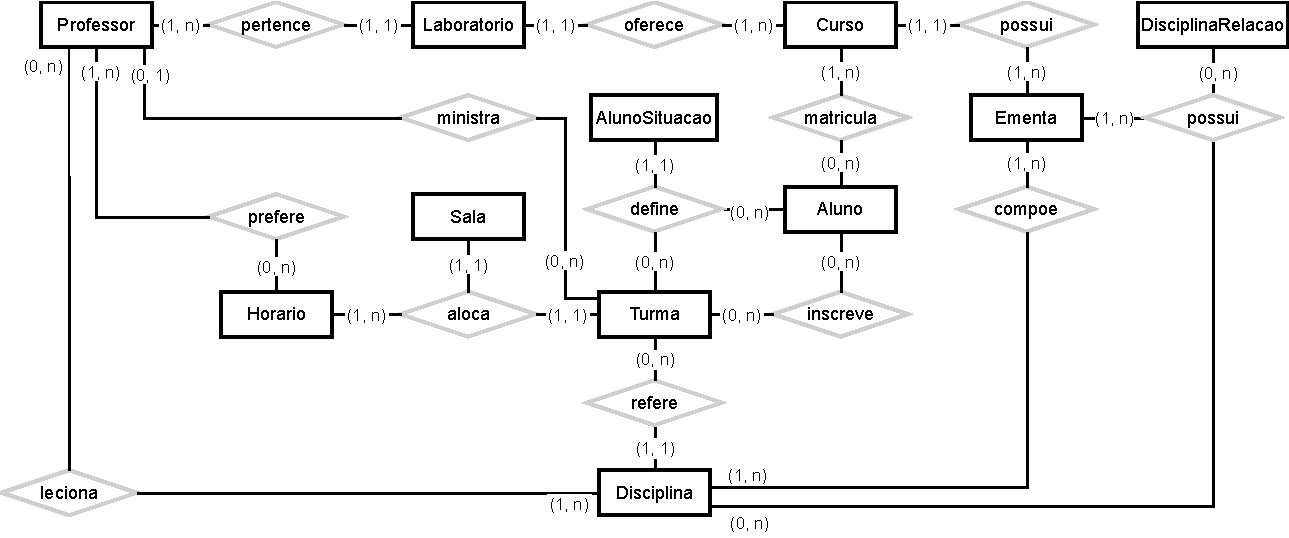
\includegraphics[width=\textwidth]{files/img/2.02!4-modelagem/Diagrama ER-Conc. Card.drawio}
\end{MyCenteredFigure} % Diagrama Conceitual

O diagrama conceitual foi elaborado utilizando a ferramenta \LinkToURL{https://www.drawio.com}{draw.io} citada na metodologia e ilustra as relações entre diversas entidades presentes na realidade da UENF. O emaranhamento presente no diagrama ilustra a complexidade envolvida na criação de uma grade horária, onde diversas entidades se relacionam entre si.

Como principais apontamentos, podemos citar a parte principal do modelo que é a alocação de turmas. Ela, como já descrito, envolve a correlação entre alunos de diferentes cursos, professores, disciplinas, salas e horários. Além disso, também é possível notar a presença de entidades que não são diretamente relacionadas à alocação de turmas, mas que podem se mostrar úteis, como a relação entre professores e laboratórios, e a de disciplinas e ementas.

Embora o diagrama apresente uma visão mais completa de todas as interconexões possíveis, é importante ressaltar que o presente trabalho foca primordialmente na alocação das turmas para o curso de Ciência da Computação, e que a implementação do banco de dados será feita de forma a atender a essas necessidades, fazendo então uso de apenas uma parte do diagrama conceitual apresentado pela \autoref{fig:DiagramConceitual}.

\subsection{Diagrama de Entidade e relacionamento} % 4.4.1.

Neste modelo, mais enxuto, temos apenas as entidades principais, onde temos uma turma de determinada disciplina, ministrada por um professor e que ocorre em uma sala em um determinado horário.

Neste diagrama vemos as entidades principais, que são \textbf{Turmas}, \textbf{Disciplinas}, \textbf{Professores}, \textbf{Horários} e \textbf{Salas}. As propriedades escolhidas para cada entidade são compostas por uma mistura de critérios. Por exemplo, o nome do professor, o código da disciplina, e a junção de código e bloco auxiliam primordialmente na identificação real dos professores, disciplinas e salas. Já as informações ``período'', ``apelido'' e ``comment''...

E também é notável a presença da entidade \textbf{Alunos}, que se apresenta desacoplado das demais entidades. O motivo para isso é que, embora os alunos façam parte do processo de alocação de turmas, ao longo do desenvolvimento, o desenvolvimento de funcionalidades envolvendo os alunos...
